\documentclass{article}
\usepackage{amsmath,amssymb,amsthm}
\usepackage{enumerate}
\usepackage{mathtools}
\usepackage{graphicx}
\usepackage{caption}
\usepackage{bm}
\newcommand{\solution}{\noindent \textbf{Solution: }}
\newtheorem{theorem}{Theorem}
\newtheorem{question}[theorem]{Question}
\newtheorem{answer}[theorem]{Solution}
\newcommand{\myvec}[1]{\ensuremath{\begin{pmatrix}#1\end{pmatrix}}}
\let\vec\mathbf
\begin{document}
\begin{question}
	Show that the unit direction vector inclined equally to the coordinate axes is $\myvec{\frac{1}{\sqrt{3}} \\ \frac{1}{\sqrt{3}} \\ \frac{1}{\sqrt{3}}}$.
\end{question}
\solution Let $\vec{m}$ be the given unit vector such that $\vec{m}$ = $\myvec{m_x \\ m_y \\ m_z}$.Let $\vec{e}_1=\myvec{1 \\ 0 \\ 0}$, $\vec{e}_2=\myvec{0 \\ 1 \\ 0}$ and $\vec{e}_3=\myvec{0 \\ 0 \\ 1}$ be the direction vectors of the coordinate axes.
As $\vec{m}$ is a unit vector, so $||\vec{m}||=1$ and also we are given is that $\vec{m}$ is inclined equally to the coordinate axis, 
\begin{equation}
\vec{e}_1^T\vec{m} =\vec{e}_2^T\vec{m}=\vec{e}_2^T\vec{m}
\end{equation}
Now, $(1)$ implies 
\begin{equation*}
\vec m_x =  \vec m_y = \vec m_z
\end{equation*}	
Thus,
\begin{equation}
\vec m = \myvec{m_x \\ m_x \\ m_x}
\end{equation}
Also, we know that $||\vec{m}||=1$ and by $(2)$, we have
\begin{equation*}
\sqrt{\vec{m_x}^2 + \vec{m_x}^2 + \vec{m_x}^2} = 1 \quad \implies
\vec{m_x} = \frac{+}{} \frac{1}{\sqrt{3}}
\end{equation*}
Taking, the positive sign, we see that  $\vec{m}$ = $\myvec{ \frac{1}{\sqrt{3}} \\ \frac{1}{\sqrt{3}} \\ \frac{1}{\sqrt{3}}}$ is the unit direction vector inclined equally to the coordinate axes.\\
\begin{figure}[!htb]
	
	\centering
	
	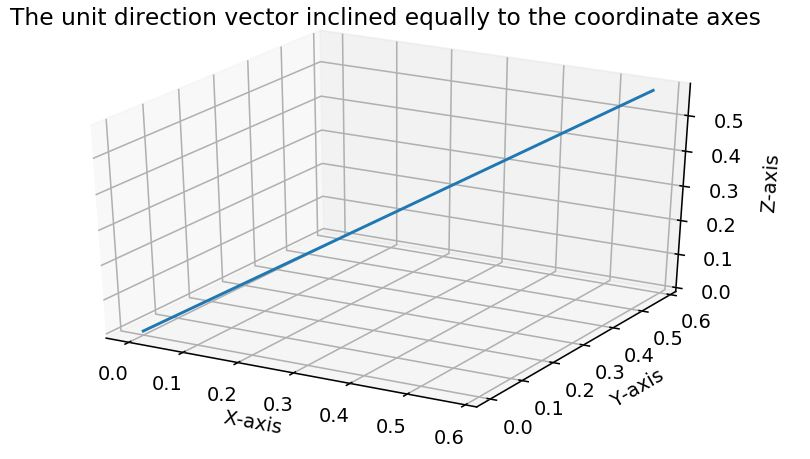
\includegraphics[width=\columnwidth]{assignment1figure.jpg}
	
	\caption{\label{fig1}}
	
	\label{fig:}
	
\end{figure}
\end{document}